\tikzset{
   plane/.pic = {
    \draw[fill]  plot[smooth, tension=0.6] coordinates {
        (-0.65,-0.9) 
        (-0.6,-0.85) 
        (-0.4,-0.75) 
        (-0.25,-0.65) 
        (-0.15,-0.5) 
        (-0.12,-0.3) 
        (-0.1,-0.1) 
        (0,0) 
        (0.1,-0.1) 
        (0.12,-0.3) 
        (0.15,-0.5) 
        (0.25,-0.65) 
        (0.4,-0.75) 
        (0.6,-0.85) 
        (0.65,-0.9)
        } -- plot[smooth, tension=0.6] coordinates {
        (0.65,-0.9) 
        (0.15,-0.91)
        (0.35,-1.1) 
        (0.37,-1.15)
        } -- plot[smooth, tension=0.6] coordinates {
        (0.37,-1.15)
        (0,-1.12) 
        (-0.37,-1.15) 
        } -- plot[smooth, tension=0.6] coordinates {
        (-0.37,-1.15)
        (-0.35,-1.1) 
        (-0.15,-0.91) 
        (-0.65,-0.9) 
        } -- cycle;
   }
}
\newcommand{\rvec}[1]{\ensuremath{{\boldsymbol{\underline{#1}}}}}
\newcommand{\rv}[1]{\ensuremath{{\boldsymbol{#1}}}}
\newcommand{\mat}[1]{{\ensuremath{{\mathbf{#1}}}}}

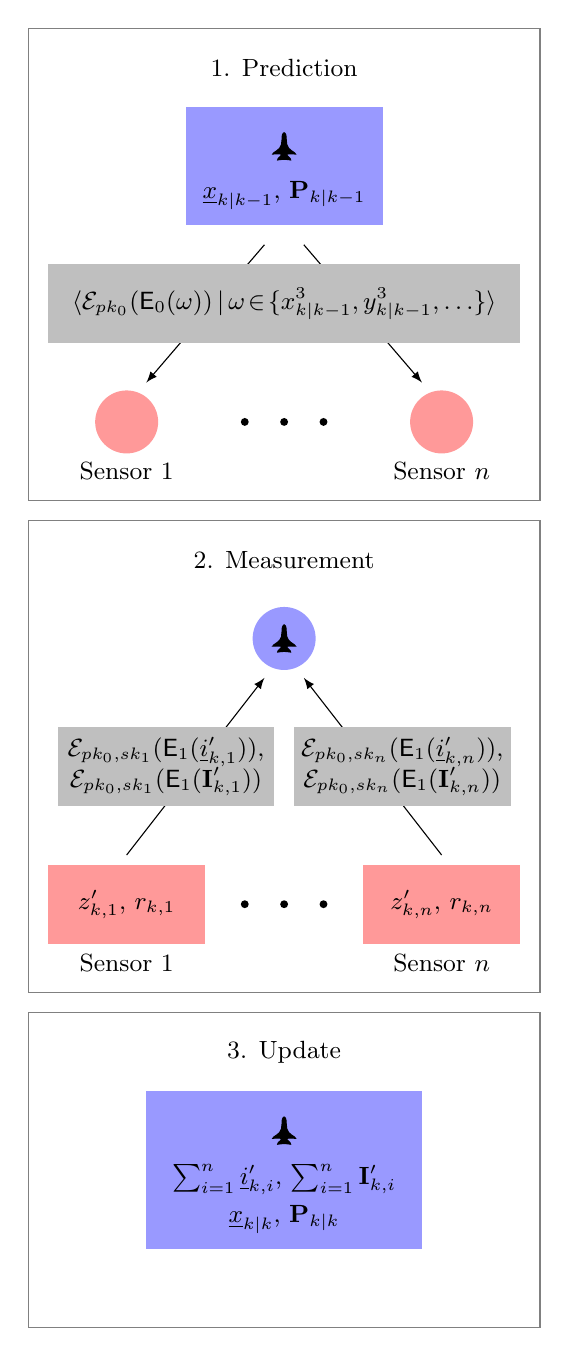
\begin{tikzpicture}[font=\small]
    % Prediction
    \draw [gray] (0,2) rectangle (6.5,8);
    \node at (3.25,7.5) {\small 1. Prediction};

    % Navigator
    \fill  [blue!40] (2,7) rectangle (4.5,5.5);
    \pic[xscale=0.22,yscale=0.3] at (3.25,6.6725) {plane};
    \node at (3.25,5.875) {$\rvec{x}_{k|k-1}$, $\mat{P}_{k|k-1}$};
    
    % Sensors
    \fill  (1.25,3) [red!40] ellipse (0.4 and 0.4);
    \node at (1.25,2.375) {Sensor $1$};
    \fill  (5.25,3) [red!40] ellipse (0.4 and 0.4);
    \node at (5.25,2.375) {Sensor $n$};
        
    \fill [black] (2.75,3) circle (0.05);
    \fill [black] (3.25,3) circle (0.05);
    \fill [black] (3.75,3) circle (0.05);
        
    % Arrows
    \draw [-latex] plot[smooth, tension=.7] coordinates {(3,5.25) (1.5,3.5)};
    \draw [-latex] plot[smooth, tension=.7] coordinates {(3.5,5.25) (5,3.5)};
    
    \fill [lightgray]  (0.25,5) rectangle (6.25,4);
    \node at (3.25,4.5) {$\langle\mathcal{E}_{pk_0}(\mathsf{E}_0(\rv{\omega})) \,|\, \rv{\omega} \!\in\! \{\rv{x}^3_{k|k-1}, \rv{y}^3_{k|k-1}, \dots\}\rangle$};
    
    
    % Measurement
    \draw [gray] (0,-4.25) rectangle (6.5,1.75);
    \node at (3.25,1.25) {\small 2. Measurement};
    
    % Navigator
    \fill  (3.25,0.25) [blue!40] ellipse (0.4 and 0.4);
    \pic[xscale=0.22,yscale=0.3] at (3.25,0.4225) {plane};
        
    % Sensors
    \fill  [red!40] (6.25,-3.625)  rectangle (4.25,-2.625);
    \node at (1.25,-3.875) {Sensor $1$};
    \fill  [red!40] (2.25,-3.625)  rectangle (0.25,-2.625);
    \node at (5.25,-3.875) {Sensor $n$};
    
    \node at (1.25,-3.125) {$\rv{z}'_{k,1}$, $\rv{r}_{k,1}$};
    \node at (5.25,-3.125) {$\rv{z}'_{k,n}$, $\rv{r}_{k,n}$};
    
    \fill [black] (2.75,-3.125) circle (0.05);
    \fill [black] (3.25,-3.125) circle (0.05);
    \fill [black] (3.75,-3.125) circle (0.05);
    
    % Arrows
    \draw [-latex] plot[smooth, tension=.7] coordinates {(1.25,-2.5) (3,-0.25)};
    \draw [-latex] plot[smooth, tension=.7] coordinates {(5.25,-2.5) (3.5,-0.25)};
    
    \fill [lightgray]  (0.375,-0.875) rectangle (3.125,-1.875);
    \node[align=center] at (1.75,-1.375) {$\mathcal{E}_{pk_0,sk_1}(\mathsf{E}_1(\rvec{i}'_{k,1}))$,\\$\mathcal{E}_{pk_0,sk_1}(\mathsf{E}_1(\mat{I}'_{k,1}))$};
    \fill [lightgray]  (3.375,-0.875) rectangle (6.125,-1.875);
    \node[align=center] at (4.75,-1.375) {$\mathcal{E}_{pk_0,sk_n}(\mathsf{E}_1(\rvec{i}'_{k,n}))$,\\$\mathcal{E}_{pk_0,sk_n}(\mathsf{E}_1(\mat{I}'_{k,n}))$};
    
    
    % Update
    \draw [gray] (0,-8.5) rectangle (6.5,-4.5);
    \node at (3.25,-5) {\small 3. Update};
    
    % Navigator
    \fill  [blue!40] (1.5,-5.5) rectangle (5,-7.5);
    \pic[xscale=0.22,yscale=0.3] at (3.25,-5.8275) {plane};
    \node at (3.25,-6.625) {$\sum_{i=1}^n \rvec{i}'_{k,i}$, $\sum_{i=1}^n\mat{I}'_{k,i}$};
    \node at (3.25,-7.125) {$\rvec{x}_{k|k}$, $\mat{P}_{k|k}$};
\end{tikzpicture}










